\documentclass[twocolumn, a4paper]{article}
\usepackage[top=1cm, bottom=1.2cm, left=1.5cm, right=1.5cm]{geometry}
\usepackage{graphicx}
\usepackage{multirow}
\usepackage{float}
\usepackage{amsmath}
\usepackage{hyperref}
\usepackage{tgcursor}
\usepackage{titlesec}
\titleformat{\section}
                {\center\scshape}
                {\thesection}{24pt}{}
\titleformat{\subsection}
                {\em}
                {\thesubsection}{20pt}{}

\setlength\intextsep{0pt}
\setlength{\columnsep}{0.6cm}

\renewcommand{\thesection}{\Roman{section}.}
\renewcommand{\thesubsection}{\Alph{subsection}.}
\begin{document}
% \setlength{\textfloatsep}{0.2cm}
% \setlength{\floatsep}{0.3cm}
\title{
    \Large\textbf{Report ``Distributed SLAM''}
	   % \vspace{1cm}
	  }
\author{
		\textbf{Bertelli Davide, Hueller Jhonny} \\
		% mat. 223718 \\
		% davide.bertelli-1@studenti.unitn.it
		% \and
		% \textbf{Hueller Jhonny} \\
		% mat. 221254\\
		% jhonny.hueller@studenti.unitn.it
	   }
\date{}
\maketitle

\textbf{
    {\em{\footnotesize{Abstract}}}%
    \small --- This report presents the results,
    solutions and implementation of a distributed SLAM system
    on a natural environment. The data were acquired through
    terrestrial agents and processed onboard. The agent were
    allowed to communicate within a certain range. Each agent
    had at its disposal a Kalmann Filter for data denoising
    and an Extendend Kalmann Filter for position estimation.
    The results shows a good accuracy in reconstructing the
    environment both in a 3D cloud and as an occupancy map.
    The estimation of the location resulted unsatisfactory.
    }

\section{Introduction}
The SLAM, acronym for Simultaneus Localisation And Mapping, is a method
employed on autonomous vehicles which allows to gather data from the
environment while localising the agent at the same time. Furthermore, it
allows to the agent to map unknown environments and update its knowledge
of the surroundings. The map resulting will then be used for further steps
in the autonomous navigation like path planning.
Agents exploiting the SLAM algorithm have been vastly employed in several
working realities which space from the industrial wherehouse menagement
up to civil indoor and outdoor agricultural solutions.
The Distributed SLAM is a variation of the SLAM method, in which multiple
agents contribute in mapping chunks of the same area to have a faster and
more precise result than the single agent case. This method aims at
exploiting at maximum the capabilities of the different agents involved
allowing to explore areas which are unexplorable otherwise.

\subsection{Problem Formulation}
The problem tried to solve in this report regards the development
of a Distributed SLAM algorithm to be deployed in natural environments.
Specifically the environment was assumed to be a forest and, by definition,
that the surroundings contain several elements with different but recurrent
shapes, like the trees. Furthermore it was kept into account the possible
presence of pits which could doom the autonomous navigation of the agents,
by posing them into an unrecoverable location. The agents employed are
assumed to be terrestrial and that their initial locations are known a
priori. The objective is to explore as long as possible the surroundings
in order to map them. The output of this process will then be a 3D cloud of
points representing the mapped environment and the occupancy map representing
the elements detected, their locations and encumbrance.
Lastly the environment it is supposed to have areas in which the GPS signal
cannot be transmitted.

\section{Adopted Models}
\subsection{Communication System}
The Communication System adopted is a Robot Network in which each agent can
transmit its data to any nearby agent within a specified communication range.
There is no master among the devices, hence a fully distributed network is
achieved. Indeed each agent acquires the data from its sensors, process them
onboard and then transmits them only if any other agent has been detected
within range. The informations transimtted consists of the point cloud
representing the environment up to the time of transmission and the
occupancy map in the local coordinate system together with its history of
poses.

\subsection{System Model}
The robot used in the development of the solution and during the simulations
is a terrestrial one. It has been modellized just for simulation purposes
and so its shape is simple event though it has the same dimensions of
a common RC car, as shown in Figure \ref{fig:Robot_dimensions}.
The sensors onboard of the agent are supposed to be, a 3D lidar, an
accelerometer and a gyroscope. Thanks to these sensors it will be possible
to map the environment around and know the tangential and radial velocities
of the agent toghether with the rotation on its axis.
For clarity, the robot has been simulated moving over the XY plane while
rotating around the Z axis.
The Lidar sensor in use aims at simulating the characteristics of the 
\href{https://www.robosense.ai/en/rslidar/RS-LiDAR-16}{RS-LIDAR-16} sensor,
but due to computation demands during simulations its horizontal resolution
has been reduced to allow reasonable computation times.
The simulated Lidar sensor has the beam origin in the center of the upper part
of the agent at an height of 0.135[m] and has the following features:

\begin{center}
\begin{tabular}{| l | c |}
    \hline
    Range & 15 meters \\
    \hline
    Horizontal Beams & 360 \\
    \hline
    Horizontal FoV & [-3.14, 3.14] radians \\
    \hline
    Vertical Beams & 16 \\
    \hline
    Vertical FoV & [-0.26, 0.26] radians \\
    \hline
\end{tabular}
\end{center}

\vspace{0.5cm}

\begin{figure}[h]
    \centering
    \includegraphics[width=8.5cm]{"../Report_images/Agent_schema"}
    \caption{Schema of the simulated agent.}
    \label{fig:Robot_dimensions}
\end{figure}

The actuators onboard of the device are supposed to be four electrical motors
posed nearby each wheel and provide traction both in the frontal and rear
axles. Furthermore, only the front wheels are supposed to rotate over
the Z axis to turn the agent in the desired direction.

\section{Solution}
\label{sec:Solution}
Our proposed solution consists in a distributed network of robots in which
each agent will acquire data from the environment and process them
autonomously. Communication is supported only for agent within a certain
distance known as a communication range.
The pipeline that each agent will execute during its lifespan can be summarized
in the following steps:
\begin{enumerate}
    \item Acquire data from the 3D Lidar sensor.
    \item Remove sensor noise from the data.
    \item Save cleaned point cloud and generate 2D occupancy map.
    \item Check if there are agents nearby. If it is the case:
        \begin{enumerate}
                \item Acquire data from nearby agents.
                \item Update local point cloud.
                \item Update occupancy map.
        \end{enumerate}
    \item Sample next location to explore using the occupancy map.
    \item Execute the maneuvers to reach the location. In this step move
          using the GPS location if available, otherwise estimate the
          location during the movement.
    \item Once arrived update the current location and repeat.
\end{enumerate}

In developing the solution to the Distributed SLAM in a forest-like
environment we had to tackle several issues, in particular the main ones
were:
\begin{itemize}
        \item Motion Model of the agent. % Differential Drive
        \item Removing Lidar Sensor noise. % KF
        \item Roadmap Generation and Path Planning.
        \item Estimating agent location in an area without GPS coverage.% EKF
        \item Possible discontinous terrain. % Pits
        \item Communication among agents.
\end{itemize}
\subsection{Motion Model}
Regarding the motion model, due to the simplicity of the shape and the inputs
at our disposal, we decided to employ the Differential Dive kinematic model
which represented our robot as a two-wheeled one with an rotation theta with 
respect to the X axis and revolving around the Z one as shown in Figure
\ref{fig:Motion_model}. Furthermore, it allowed
to control our agents motion by providing the desired tangential
and radial velocities other than specifying the wheels radius and axle
separation.
\begin{figure}[h]
    \centering
    \includegraphics[width=4cm]{"../Report_images/diffdrive_model_matlab"}
    \caption{Differential Drive example.}
    \label{fig:Motion_model}
\end{figure}
\subsection{Lidar Noise Removal}
Due to the data acquisition from a sensor it was not possible to
omit the possible presence of noise in the informations retrieved.
For this reason we assumed the presence of an additive gaussian noise in
the input stream and to counteract its effect we decided to
use a linear Kalmann Filter to estimate the true value of the data.
Specifically, the equations ruling the Kalmann Filter in use are the following.
\begin{equation}
    \hat{x} = A\hat{x} + Bu
\end{equation}
\begin{equation}
    P = APA^{-1} + Q
\end{equation}
\begin{equation}
    K = PH{HPH^{T} + R}^{-1}
\end{equation}
\begin{equation}
    \hat{x} = \hat{x} + K(Z - H\hat{x})  
\end{equation}
\begin{equation}
    P = P - KHP  
\end{equation}

Where $\hat{x}$ is the estimated state, $A$ is the state transition matrix,
$B$ is the input matrix, $u$ is the input vector, $Q$ is the process noise
covariance, $K$ is the Kalmann gain, $H$ is the observation matrix,
$R$ is the observation covariance and $Z$ is the measurement taken from the
sensor.

\subsection{Roadmap and Path Planning}
Concerning the Roadmap Generation and Path Planning issues, we decided to
make the agent chose its next location through a uniform random sample
operation over the free space areas within a maximum distance equal to the
lidar range. In this way the worst scenario would still have the agent in
a free space area. Furthermore, we also supposed that the GPS location could
incurr into some errors and so we decided to allow the agent to approximate
its location to the nearest free one through gaussian sampling in case the 
initial location would result into an occupied or invalid one. Once the
initial and arrival locations are in a free space area the agent will then
generate the roadmap necessary to reach the arrival position. The algorithm 
chosen to carry out this task is the RTT*. The choice of this algorithm has
been lead due to its ability to find paths even through narrow apertures
between detected objects and also due to its inner nature of being a tree
graph which will depart from the initial location, exploring and re-wiring
itself until it reaches its goal. This latter behaviour has been decisive in
the choice, especially against the common PRM which will randomly sample all
the environment generating a bunch of useless data. Lastly, to ensure a
certain fluidity in the agent motion we constrained the sample of the
next location using spatial boundaries like the ranges of arriaval rotation,
the minimum and maximum x-y values.

\subsection{Agent Position Estimation}
Regarding the position of the agents in use we are using their absolute
location in the space and we keep it updated thanks to the data retrieved
by the GPS onboard. Unfortunately in natural environment it is not always
possible to rely on these measurement, so we needed also a way in which to
estimate the location of the robots relying only on the measurements retrieved
and the motion model of the robot itself. To achieve this task we decided
to employ an Extended Kalmann Filter which is specific for non-linear models.
Its strength is due to the linearizations through derivation of the non-linear
functions ruling the measurements acquisition and the states transition.
The equations ruling its behaviour are the same of the linear Kalmann Filter,
with the only difference that the covariance of the state and the observation
are computed deriving the respective functions.

\subsection{Discontinuous Terrain}
Working on a natural environment must also imply that the surface on which the
agents will move cannot be homogeneous and so the presence of pits or holes
must be taken into account.
For this reason in the processing of the 3D point cloud coming from the Lidar
we appended some lines of code which will perform an automatic detection
of the points representing the ground through the SMRF algorithm and
then will further classify these points in pits and non-pits depending by
their Z distance from the origin of the Lidar beams. Doing so we can ensure
that the agents will avoid such detected pits by embedding their points into
the occupancy map generated by the original point cloud, tricking the robots
into observing the pits as occupied space.

\subsection{Communication}
Being our system distributed over a moltitude of agents it is also necessary
to establish some procedure of communication. In particular we have assumed
that two arbitrary agents can share informations if they are within a certin
communication range. To simulate this behaviour we supposed that the agents
has onboard some kind of sensor which act as a proximity one telling at
which distance and orientation there is an agent. These informations have
been practically provided to the agents through a third kind of agent
which is omniscent regarding the global positioning of the other agents
and that can access their inner class data. It is important to point out
that this is a mere program and not a simulated sensor itself.
Thanks to its presence it will then be possible to virtually share the data
between the existing agents.

\section{Implementation Details}
In this section of the report will be presented how the system has been
simulated and implemented, together with its architecture.
\subsection{Software In Use}
For the development of our solution we used local machine running Matlab R2021b
for creating and running
the scripts ruling the agents, performing the data processing and allowing the 
connection to the simulation environment. This latter one is 
generated by the simulation software Gazebo v11.11 which provided the
pyshical constraints of the objects and environment dynamics. The worlds over
which the simulation runs have been manually created using Blender v3.2.
Furthermore the bidirectional communication between Matlab and Gazebo has
been possible using the ROS framework integrated with Gazebo, specifically
ROS Noetic v1.15.14.
The software architecture is summarized and proposed in Figure \ref{fig:S_Arch}.
\vspace{0.5cm}
\begin{figure}[h]
    \centering
    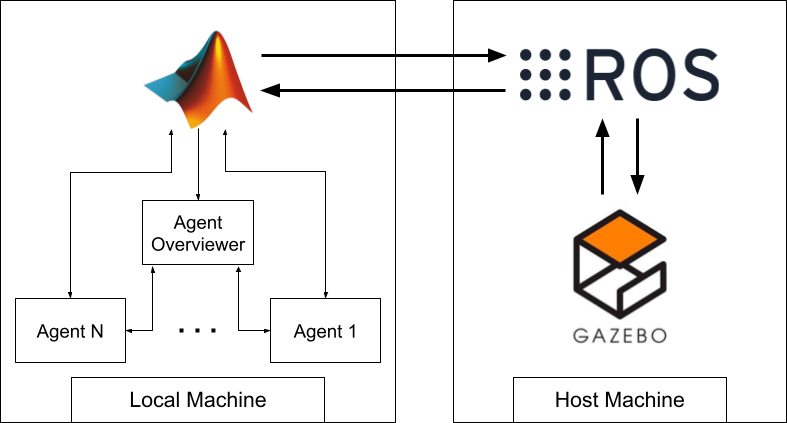
\includegraphics[width=8.5cm]{"../Report_images/Simulation_Architecture.png"}
    \caption{Schema of the Simulation Architecture}
    \label{fig:S_Arch}
\end{figure}
\subsection{Software Components}
As Shown in Figure \ref{fig:S_Arch} matlab rules over two classes of objects:
the agents and the agentOverviewer. The agent class is the one responsible 
for the data acquisition and processing, roadmap generation, path planning and
maneuver execution. This class communicate through matlab using the ROS
framework to retrieve sensible data from the simulation in gazebo, this data
are the simulated 3D Lidar output and the odometry.
The other class ruled by the Matlab environment is the agentOverviewer which
accesses all the properties of the agents existing and exploits their
knowledge and methods to share data with all the other agents which 
satisfies the communication criterion. It is important to notice how this
class do not interfaces directly to the simulation through matlab, but
delegates the agents into taking the data it needs from the simulated
environment. This behaviour is used to simulate a digital proximity sensor
which is onboard of each agent. Lastly, this class also embeds the informations
regarding which areas of the global map do not allow for GPS data retrival
and forces the agents to estimate their locations.

\section{Results}
In this section of the report will be shown the results achieved by our
solution. For sake of clarity we will present results regarding the different
steps of the workflow executed by each agent and lastly the global results.
We will also put focus on the issues tackled in Section \ref{sec:Solution}.
Specifically we will start discussing about the 3D Lidar data denoising, then
about the pits detection, later on the sharing data among the agents,
thereafter about the roadmap generation and lastly about the estimation
of the agent location in areas without GPS.
\subsection{Lidar Data Denoising}
In processing the incoming 3D point cloud from the Lidar sensor we decided
to estimate its true values against the noise exploiting a Linear Kalmann
filter, but before testing it directly against the Lidar data we wanted to
have a clear understanding of the goodness of our implementation. For this
reason we generated samples from a sine function to which we have summed
a gaussian noise with 0 mean and 0.1 variance. On these samples we applied
the Kalmann Filter and retained its estimates. The result can be seen in
Figure \ref{fig:KF_sine} and Figure \ref{fig:KF_sine_err}. In the first
figure we can observe how the estimated values in output from the Kalmann
Filter still exhibit the noise behaviour, but correctly follows the
curves of the sine wave. In particular by increasing the values of the 
observation covariance matrix in the Kalmann Filter it
is possible to achieve a 
smoother behaviour of the estimates, but after several trials we decided
that its current value, 0.3, was granting us an acceptable error, as shown
in the second figure. The error function used to estimate the goodness
of the estimation is the following:
\begin{equation}
    error = ||\hat{x} - x||
\end{equation}
in which $\hat{x}$ is the current estimate and $x$ is the true value.
\vspace{0.5cm}
\begin{figure}[h]
    \centering
    \includegraphics[width=8.5cm]{"../Report_images/Denoising_KF_sine"}
    \caption{Linear Kalmann Filter test over a sine wave.}
    \label{fig:KF_sine}
\end{figure}
\vspace{0.5cm}
\begin{figure}[h]
    \centering
    \includegraphics[width=8.5cm]{"../Report_images/Denoising_KF_sine_error"}
    \caption{Linear Kalmann Filter test over a sine wave error. The red line is
             the mean.}
    \label{fig:KF_sine_err}
\end{figure}
Once we were satisfied of these results we applied the Kalmann Filter to the
data coming from the Lidar. In order to achieve satisfactory results we had
to tune up again the observation covariance and process noise matrix, 
respectively of value 0.3 and 0.1. The tests have been carried out on
Lidar data having gaussian noise with 0 mean and variance of 0.01 and 0.1, which
resulting point clouds are shown in Figures \ref{fig:KF_cloud_01} and
\ref{fig:KF_cloud_1}. The original noisy cloud matrix has been omitted for the
clarity of the results.
\vspace{0.5cm}
\begin{figure}[h!]
    \centering
    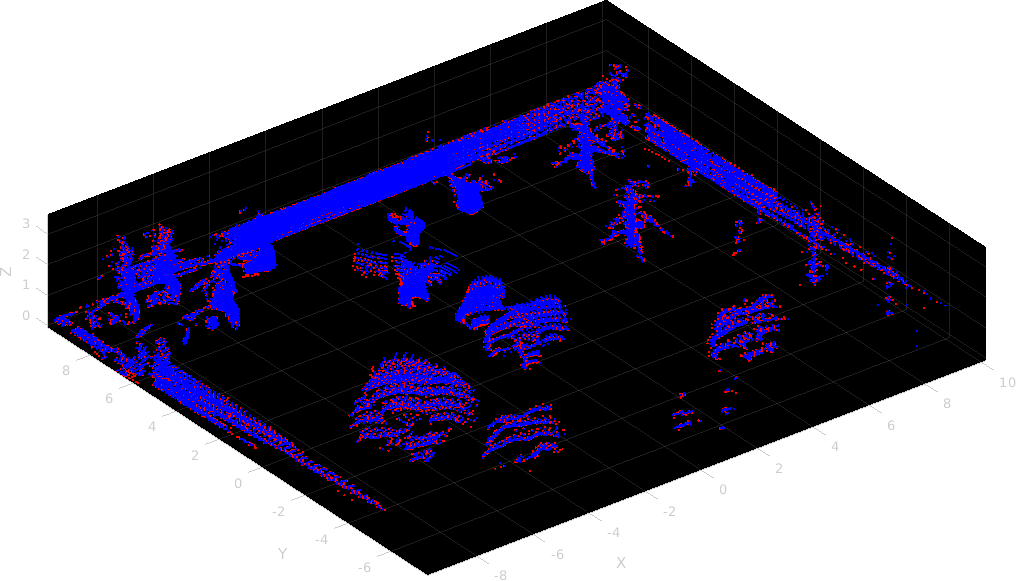
\includegraphics[width=8.5cm]{"../Report_images/Cloud_01_estimation_KF.png"}
    \caption{Estimated point cloud from gaussian noise having 0 mean and 0.01
             variance, in red. Noiseless point cloud in blue.}
    \label{fig:KF_cloud_01}
\end{figure}
\vspace{0.5cm}
\begin{figure}[h!]
    \centering
    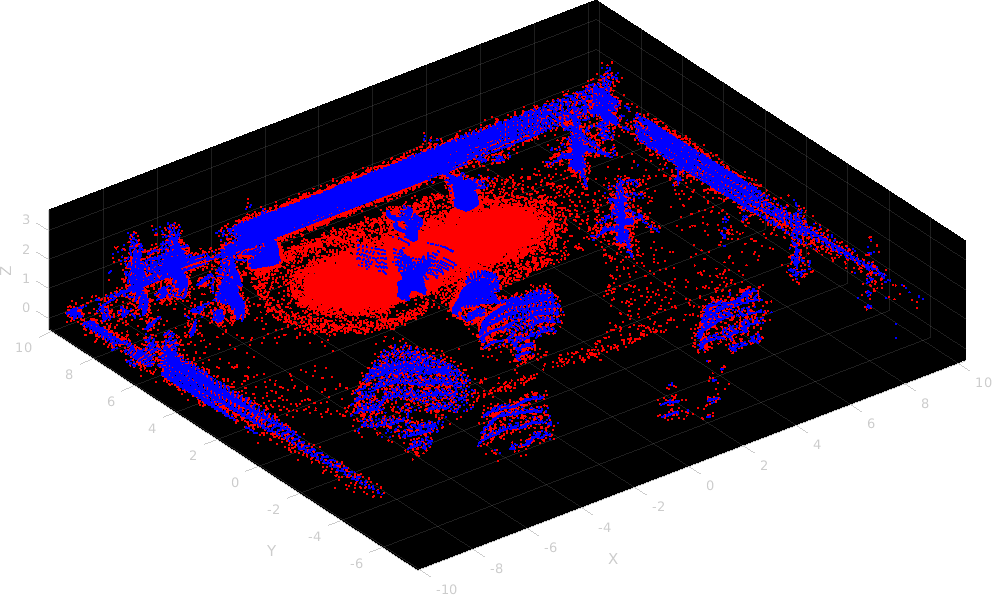
\includegraphics[width=8.5cm]{"../Report_images/Cloud_1_estimation_KF.png"}
    \caption{Estimated point cloud from gaussian noise having 0 mean and 0.1
             variance, in red. Noiseless point cloud in blue.}
    \label{fig:KF_cloud_1}
\end{figure}
\newpage
As it is possible to notice from the figures, we have that in both cases the
Kalmann Filter in use is able to correct the noisy input and produce a result
not so different from the truth value, in blue. In particular the process
seems to fail in Figure \ref{fig:KF_cloud_1} in which a huge area of the
ground is shown in red. This error is partially due to the Kalmann Filter
itself in estimating the position of the points nearby the ground, but the
majority of the fault goes to the SMRF algorithm run to detect the ground
which will then be removed from the point cloud. This error also shows how
a variance of 0.1 in the input data is able to generate such foggy data to
challenge the detection of the ground.
Following the needs to have a measure of the goodness of the estimation
we tried to compute an estimation error, but due to the misalignment of the
estimated points locations with the truth values locations, we had to crop
the estimated points resulting into a bayased error plot. Anyway such plot
can still offer some hints on the goodness of the estimation.
The error plots for both cases are shown in Figures \ref{fig:KF_err_01} and
\ref{fig:KF_err_1}. The error function in use is the following:
\begin{equation}
    error = RMSE(||(\hat{x} - x)||)
\end{equation}
Indeed we can observe that in the first figure the error rises but then 
saturates, while in the second figure its behaviour results quite jittery.
\newpage
%\vspace{0.5cm}
\begin{figure}[h!]
    \centering
    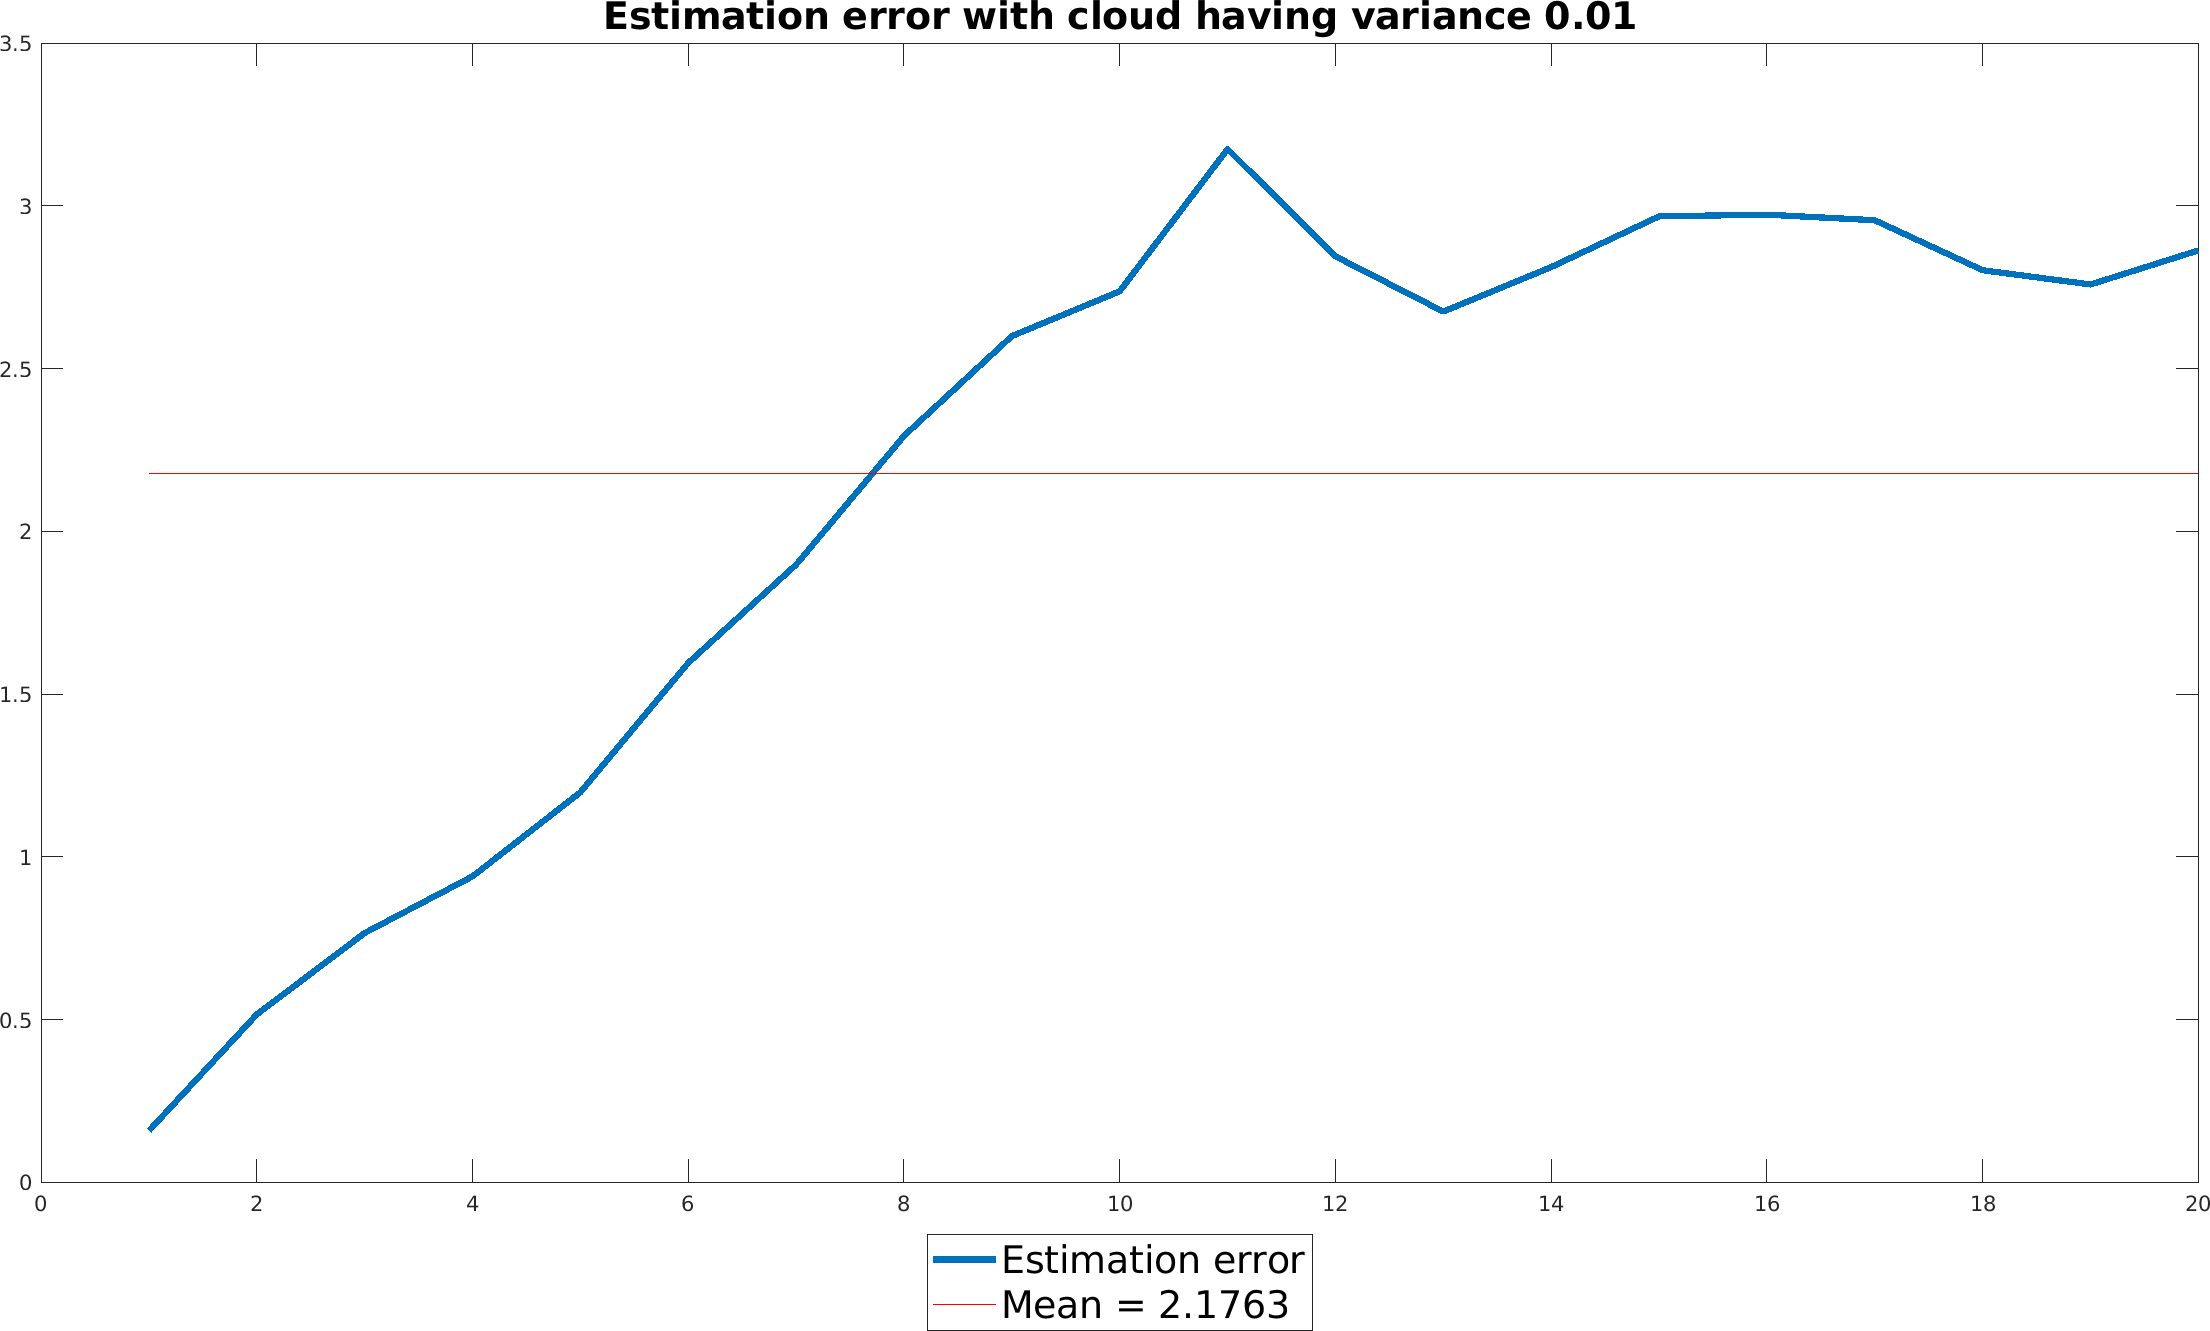
\includegraphics[width=8.5cm]{"../Report_images/Denoising_KF_cloud01_error.png"}
    \caption{Estimation error for 0.01 variance. The red line is the mean.}
    \label{fig:KF_err_01}
\end{figure}
\vspace{0.3cm}
\begin{figure}[h!]
    \centering
    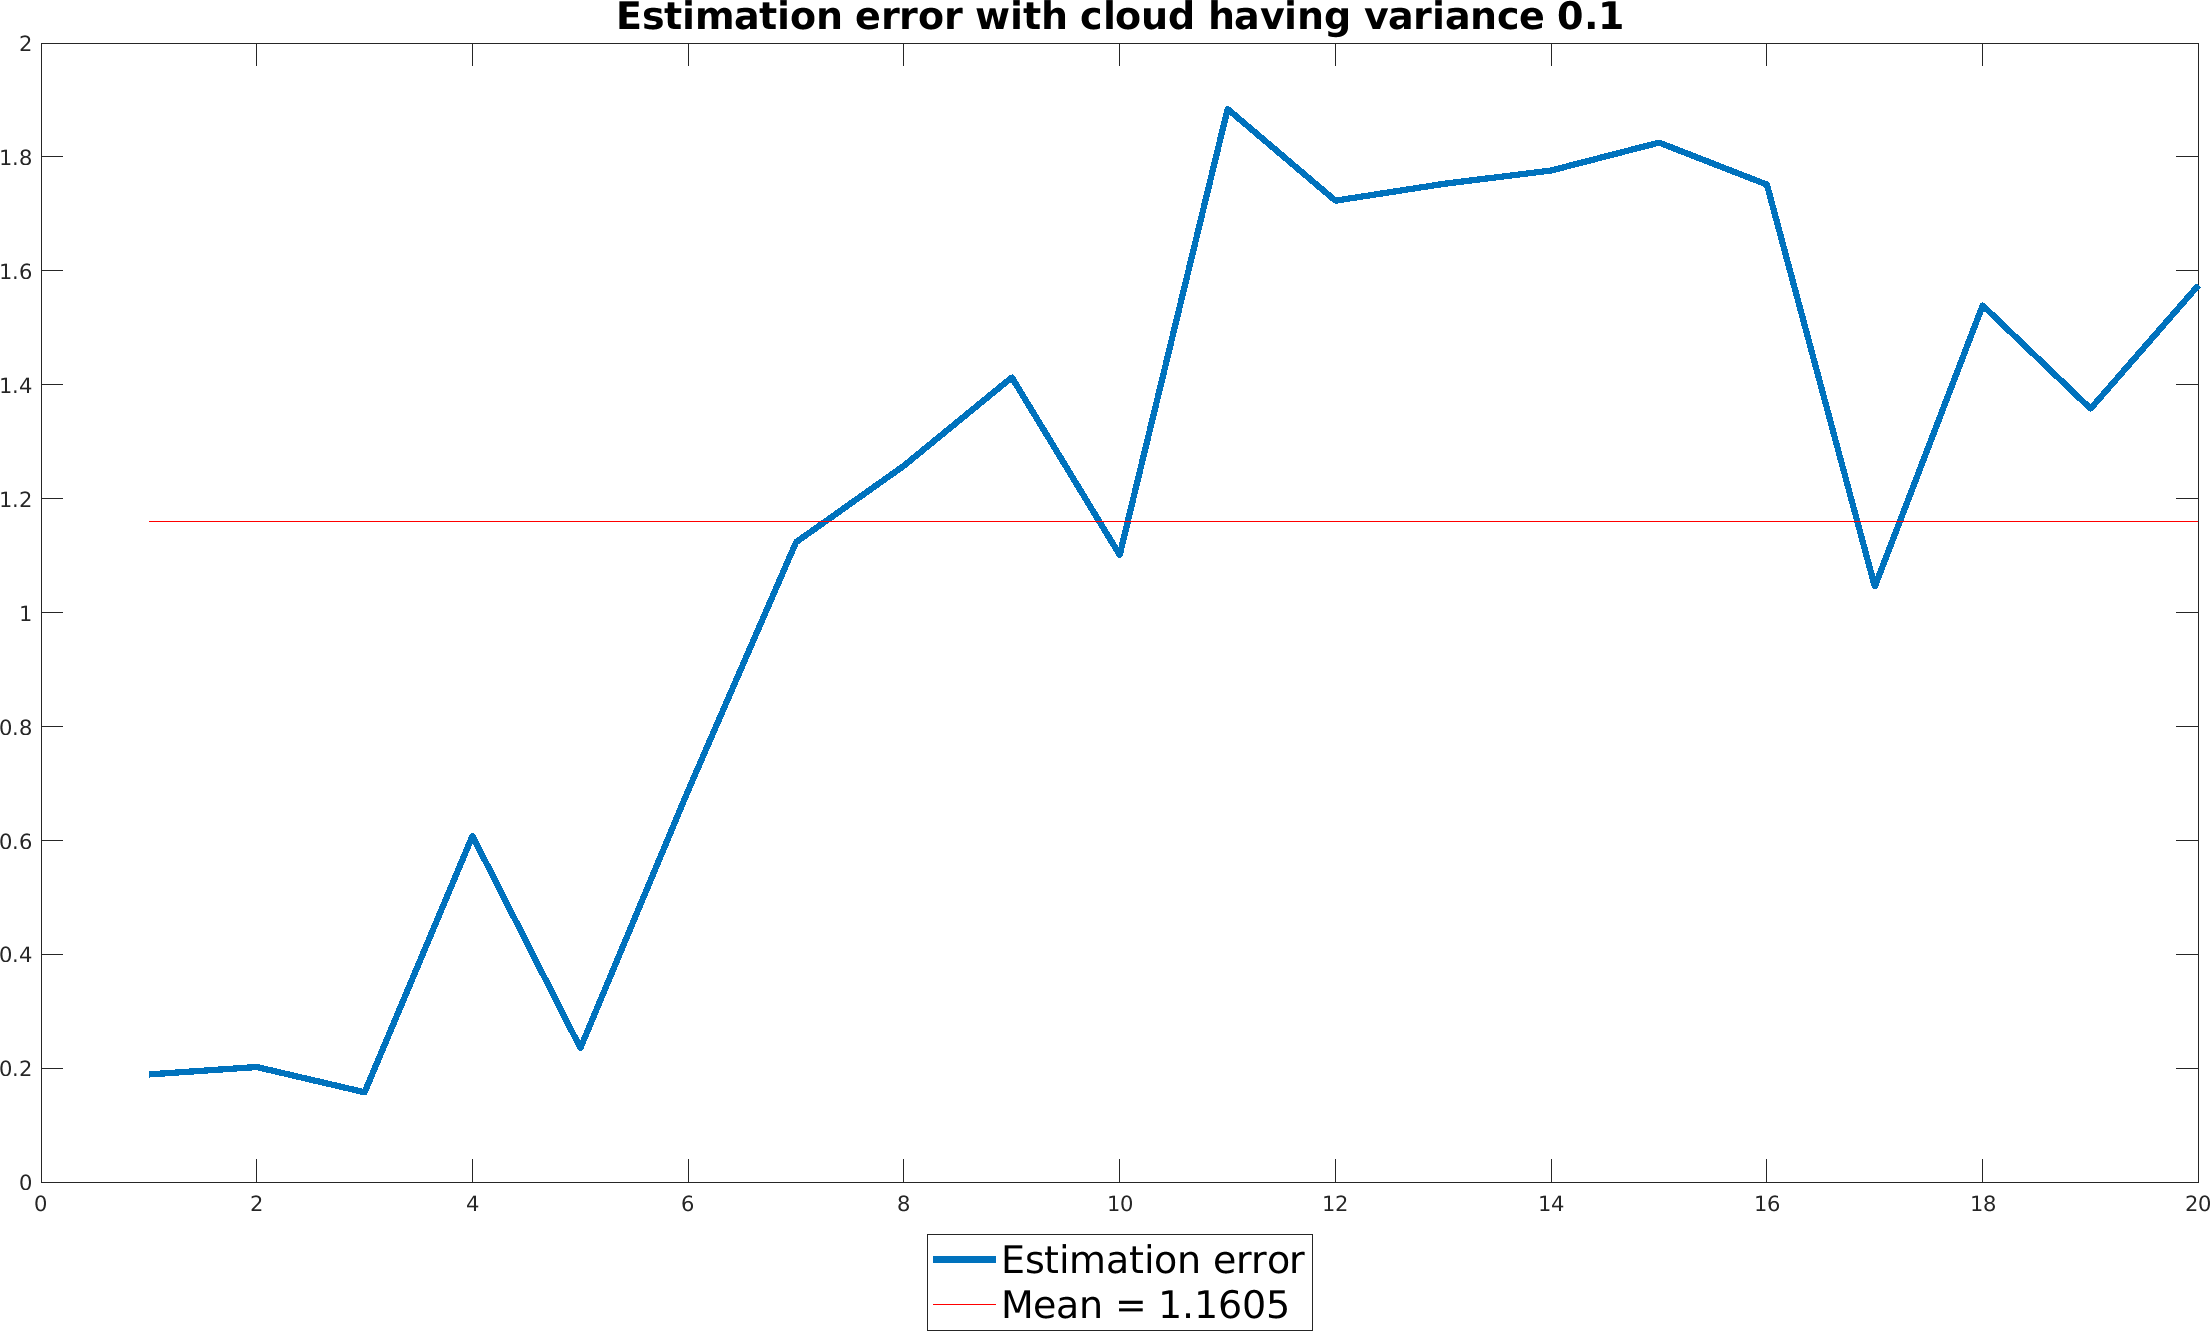
\includegraphics[width=8.5cm]{"../Report_images/Denoising_KF_cloud1_error.png"}
    \caption{Estimation error for 0.1 variance. The red line is the mean.}
    \label{fig:KF_err_1}
\end{figure}

\subsection{Pits Detection}
As stated in Section \ref{sec:Solution} the pits detection is a core
functionality of the solution allowing to avoid unrecoverable states. For
this reason from the point clouds it has been extracted the ground
for detecting the pits it contains. The criterion used in
identifying them is their distance on the Z axis,
specifically a point has been classified as a pit one if its location
on the Z axis was lower or equal than minus two times the height of the agent.
Once the detection ends the points are removed from the ground and
added to the occupancy map as occupied space.
The results of this approach can be seen in Figures \ref{fig:cloud_pits} and
\ref{fig:occupancy_pits}.
\begin{figure}[h!]
    \centering
    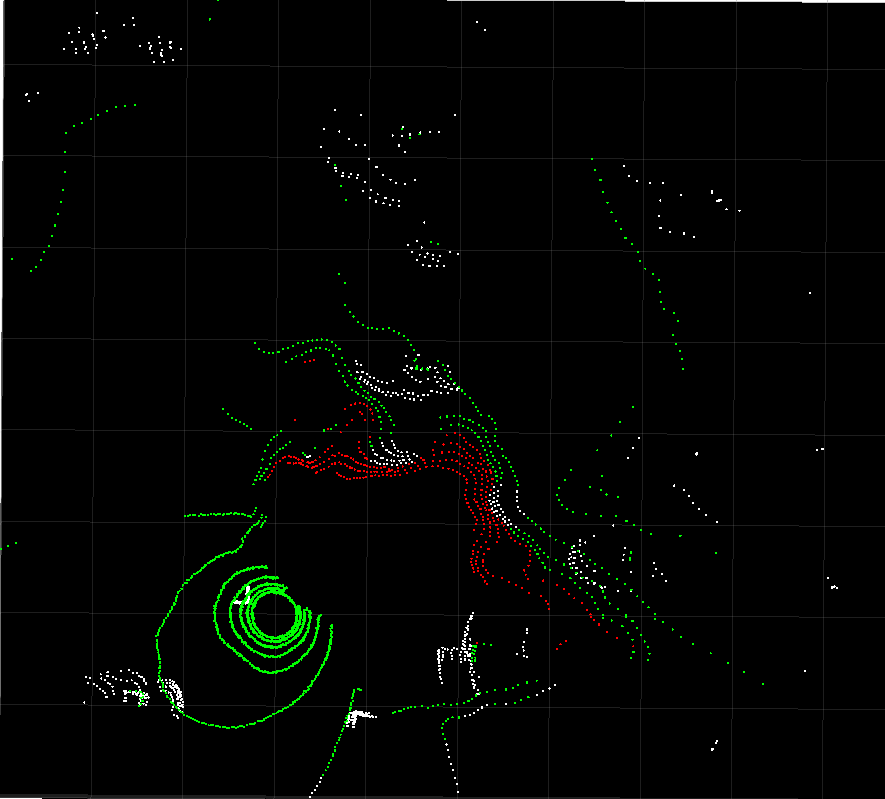
\includegraphics[width=8.5cm, height=6.5cm]{"../Report_images/Pits_3D_cloud.png"}
    \caption{Colour mapped point cloud: in gray the natural
             elements, in green the ground and in red the pits.}
    \label{fig:cloud_pits}
\end{figure}
% \vspace{0.5cm}
\begin{figure}[h!]
    \centering
    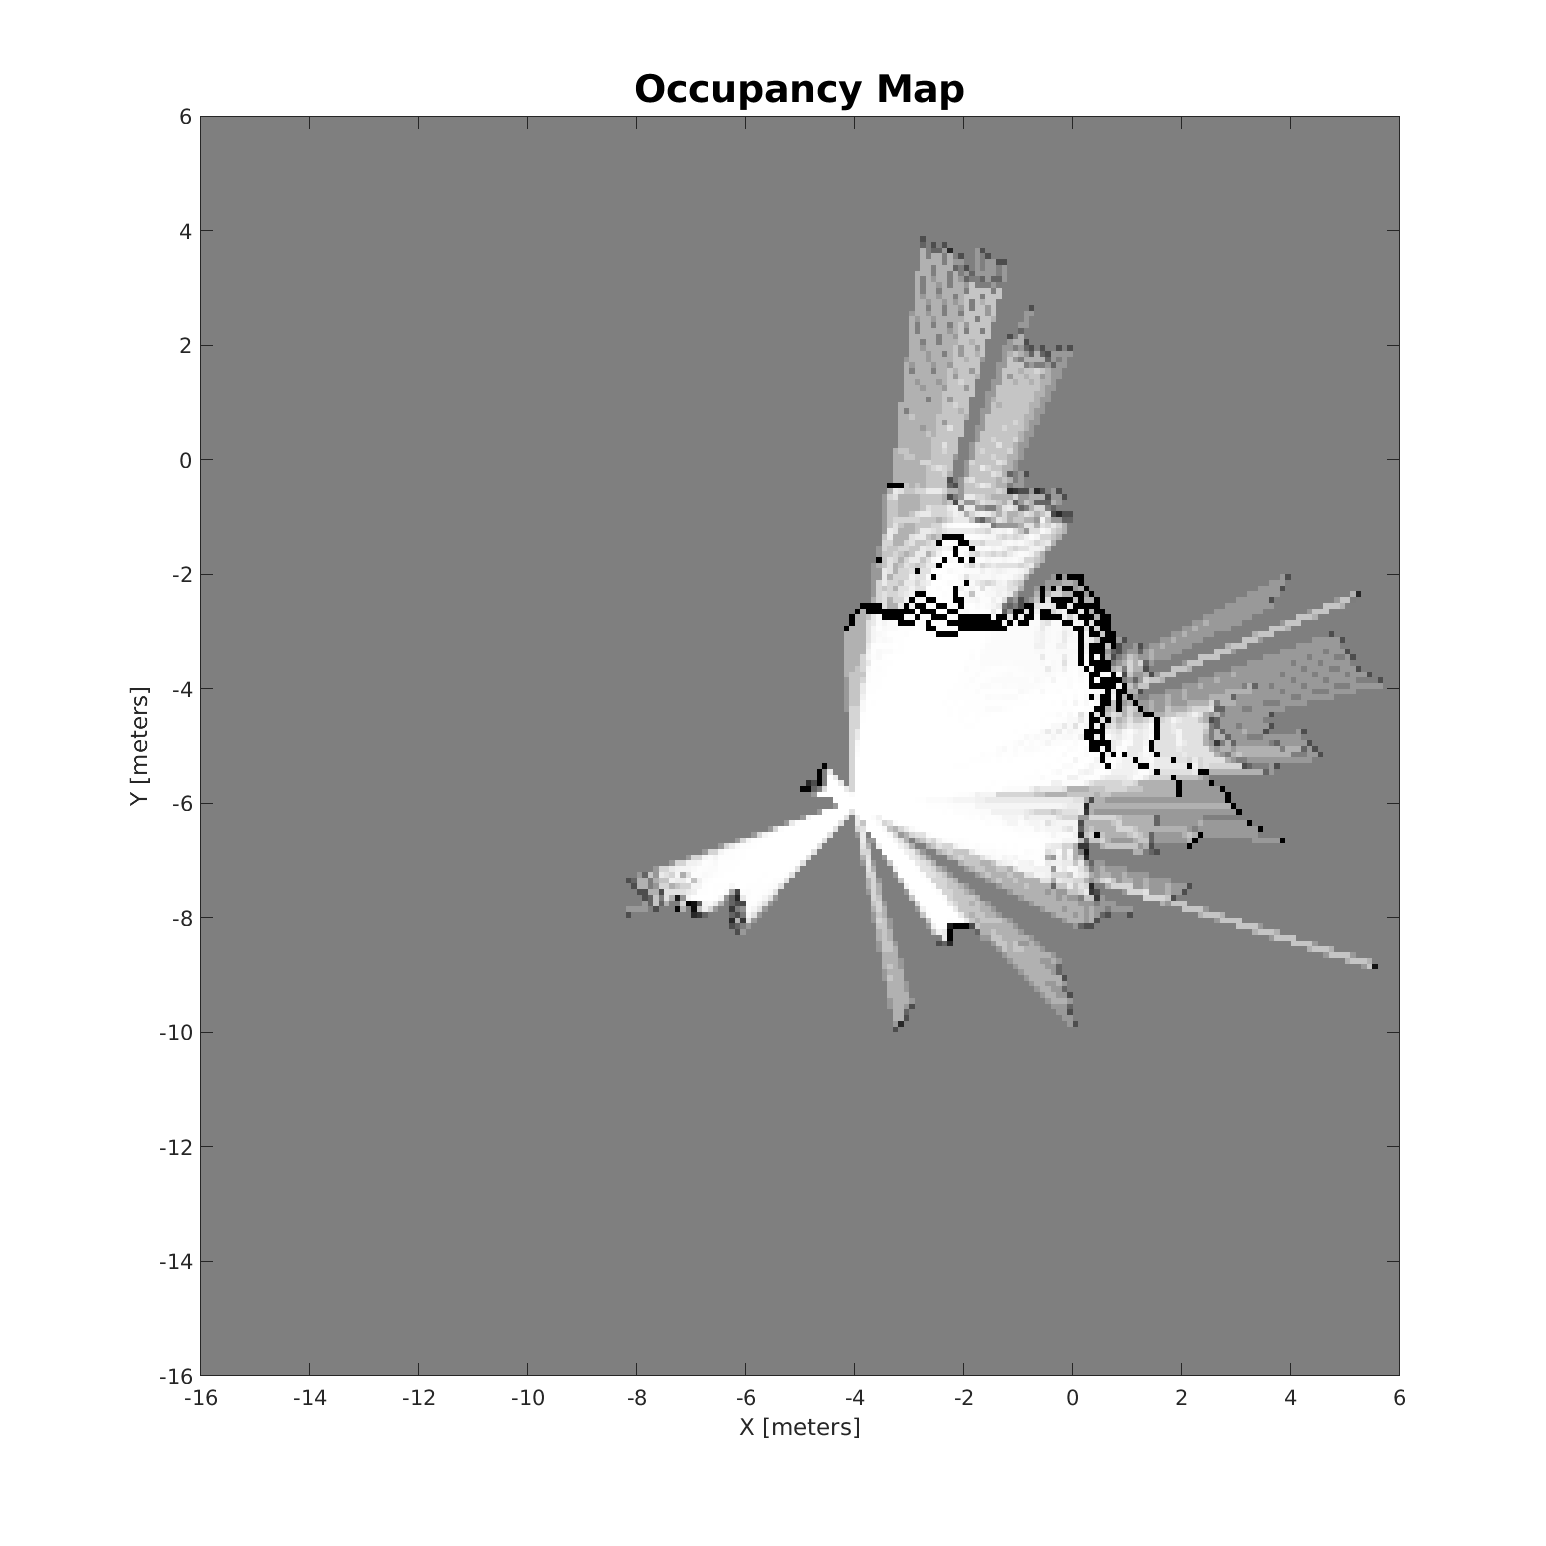
\includegraphics[width=8.5cm]{"../Report_images/Occupancy_pits.png"}
    \caption{Occupancy map updated with the pits points, upper right.}
    \label{fig:occupancy_pits}
\end{figure}

\subsection{Sharing Data Among Agents}
The sharing of data among the agents has been carried out by querying the
agentOverviewer class for stating the agents nearby and providing the
data of those agents within the communication range to the asking agent.
The only issue in this process is the merging and alignment of the data
contained in the occupancy maps of the two agents into one map. Thanks to
the usage of the absolute coordinates of each agent in simulation and to
the role of the agentOverviewer in providing also this information, the
resulting merged map is immediately done. Following are the results before
and after merging of two agents in opposite locations of the map and having
also different orientations. We can notice how in both cases the resulting
map is not affected by the different pose of the agents thanks to a 
preventive homogeneous transformation over the point cloud data into global
coordinates performed autonomously by each agent before sharing their data.
Instead the transformation of the data in the occupancy map is performed
after the sharing by the receiving agent. In Figures \ref{fig:occ_single} and
\ref{fig:occ_merged} we can observe the before and after merging in the
occupancy cloud for Agent 2, while in \ref{fig:cloud_merged} we can see
the resulting merged cloud point.
\vspace{0.5cm}
\begin{figure}[h!]
    \centering
    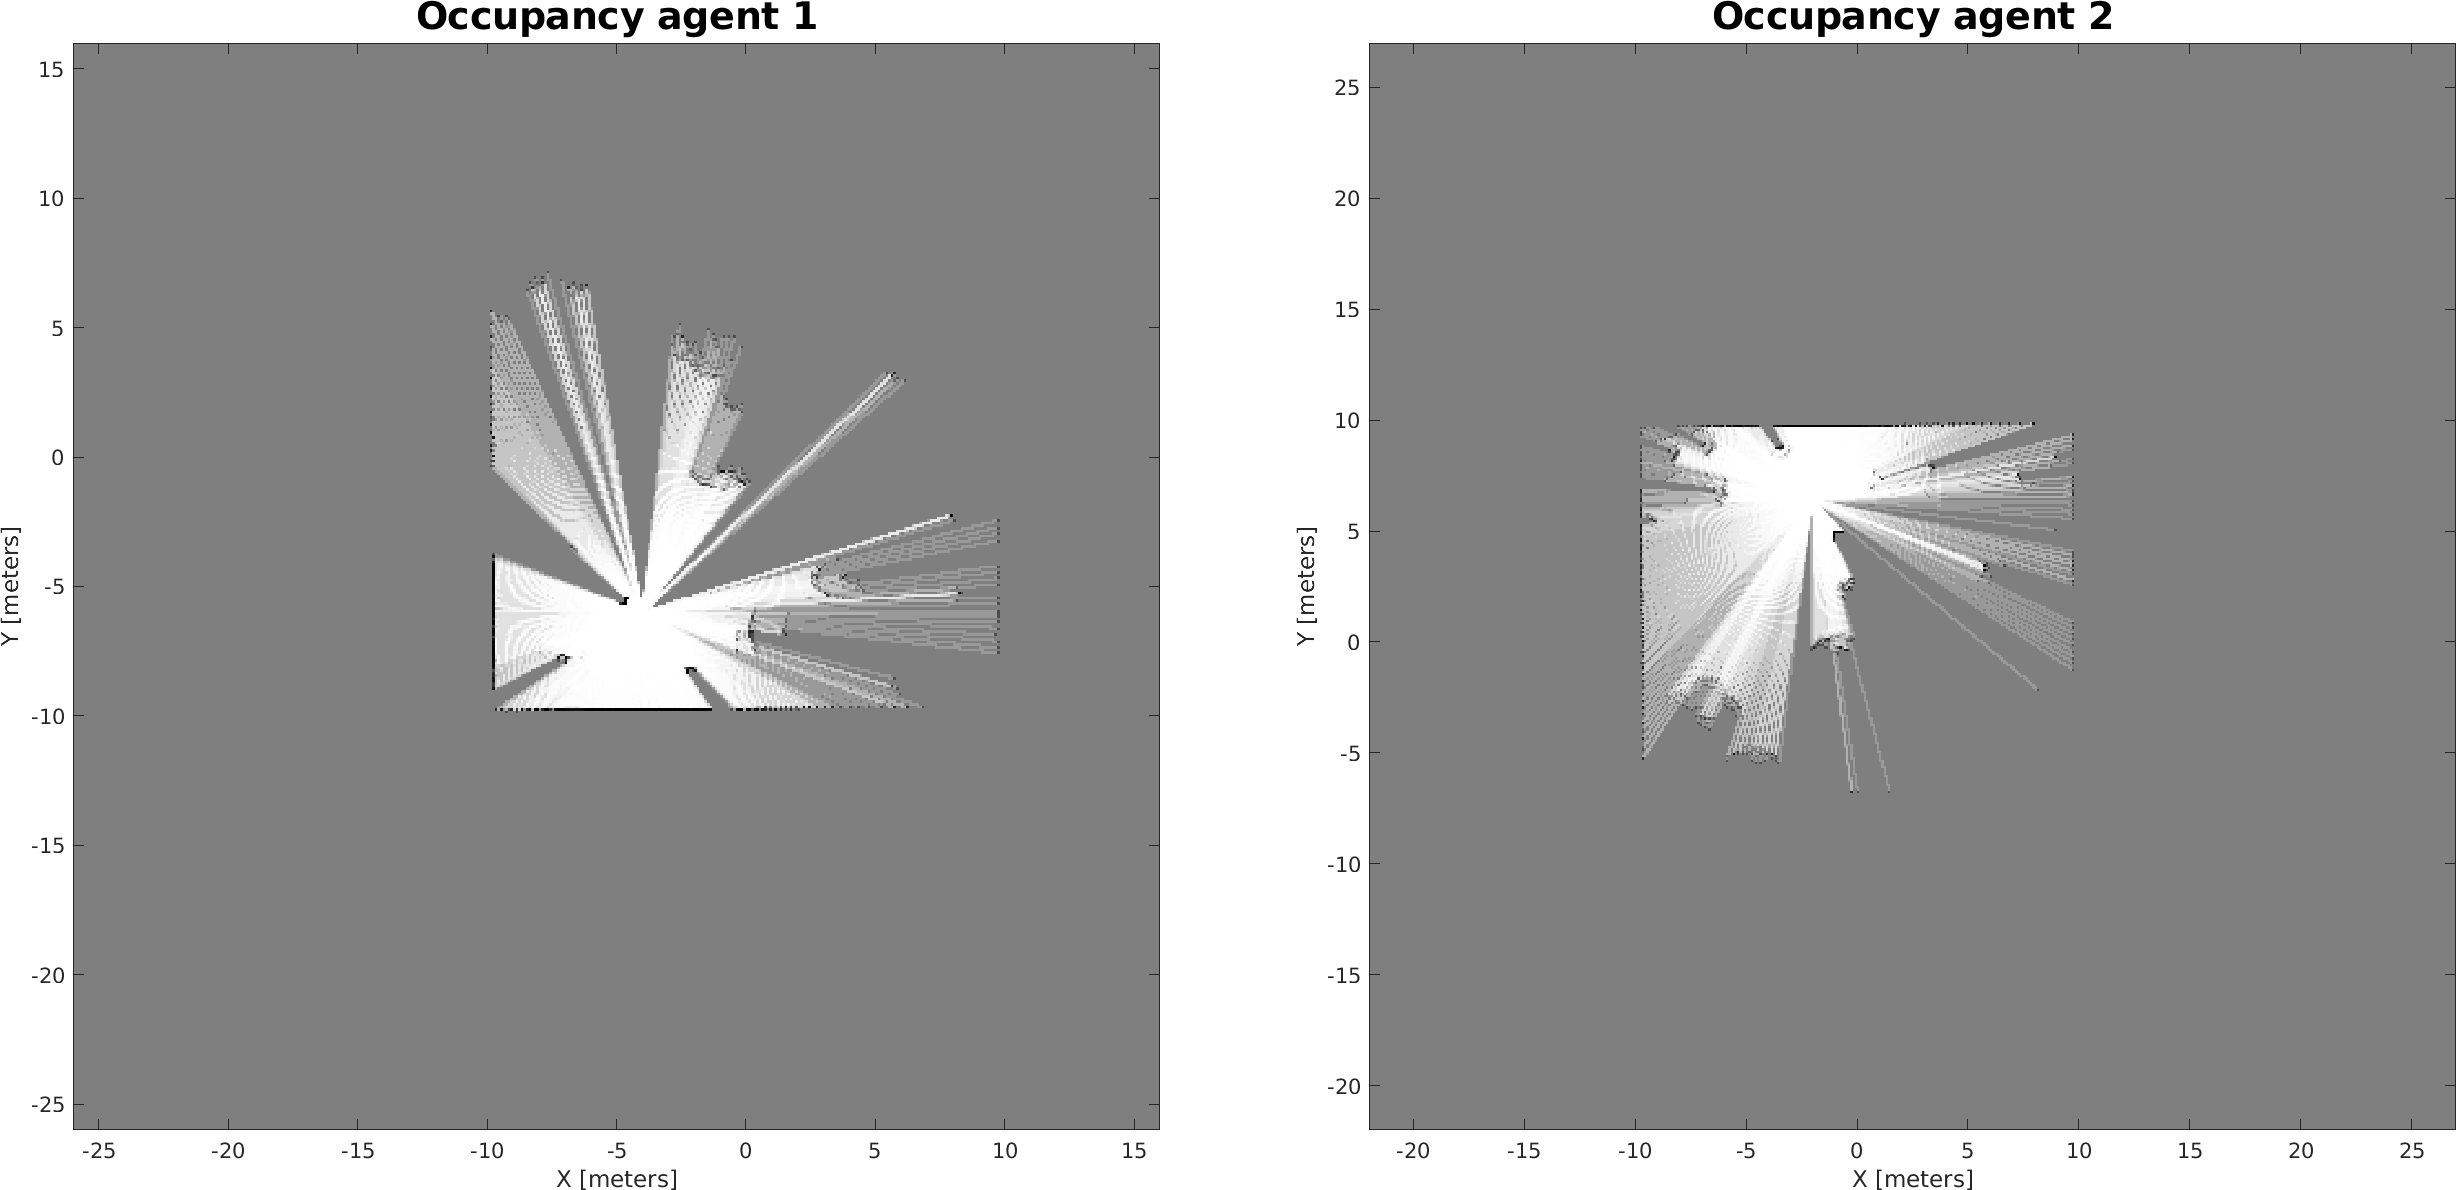
\includegraphics[width=8.5cm]{"../Report_images/Single_occupancies.png"}
    \caption{Single occupancy map for the agents in simulation.}
    \label{fig:occ_single}
\end{figure}
\vfill
% \vspace{0.5cm}
\begin{figure}[h!]
    \centering
    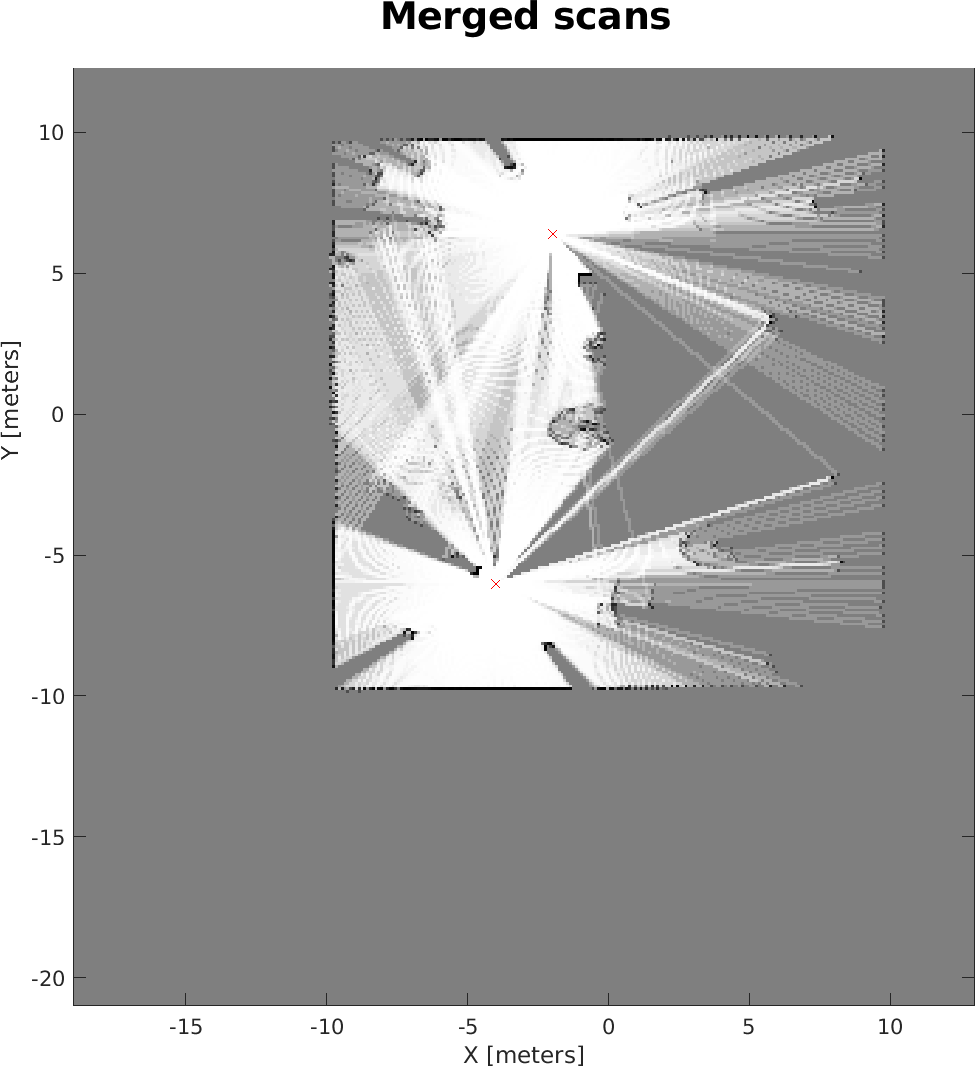
\includegraphics[width=8.5cm]{"../Report_images/Merged_occupancies.png"}
    \caption{Merged occupancy map for Agent 2. The red crosses are the
             absolute postions of the agents from which the data were
             acquired.}
    \label{fig:occ_merged}
\end{figure}
\begin{figure}[h!]
    \centering
    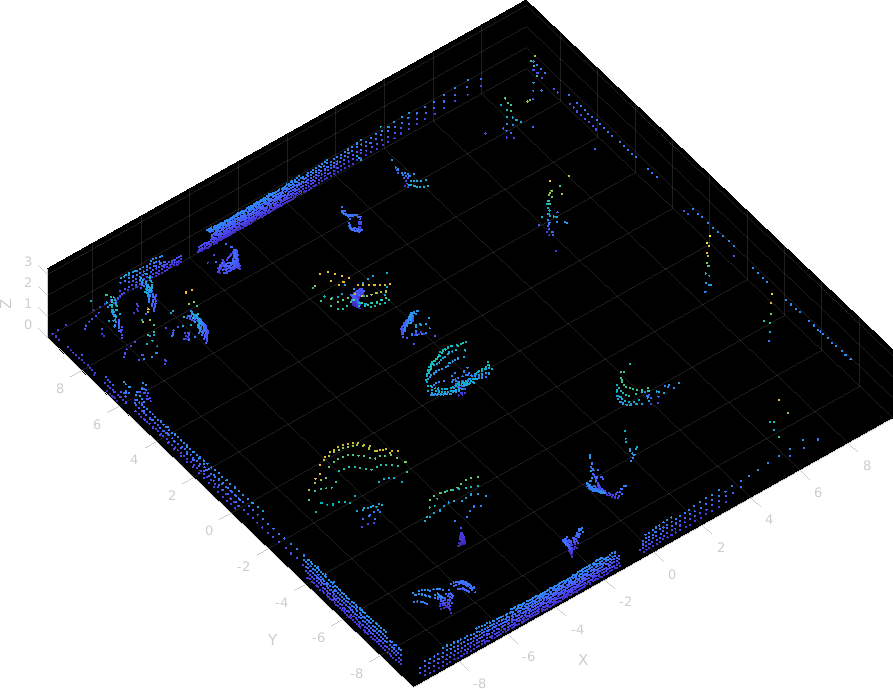
\includegraphics[width=8.5cm]{"../Report_images/Merged_cloud.png"}
    \caption{Merged point cloud for Agent 2.}
    \label{fig:cloud_merged}
\end{figure}

\subsection{Roadmap Generation}
As stated in Section \ref{sec:Solution} the roadmap computation is
performed by randomly sampling the next location in which to perform the
scanning of the environment and computing the path to this position exploiting
the RTT* algorithm. The result of this process can be observed in Figure
\ref{fig:Roadmap_ex}. In it we can see that the occupancy map has been
inflated in order to avoid collisions with the nearby objects and on top
of that the tree to the goal location has been computed.

\newpage
\begin{figure}[h]
    \centering
    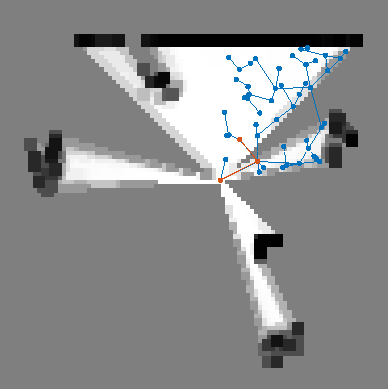
\includegraphics[width=5cm]{"../Report_images/Roadmap.png"}
    \caption{Computed roadmap, in blue, and selected path to the next location
             red. Starting point is in the center, arrival point is on top.}
    \label{fig:Roadmap_ex}
\end{figure}

\subsection{Agent Location without GPS}
The last issue tackled in Section \ref{sec:Solution} is the one of estimating
the current absolute pose of an agent employing the Extended Kalmann Filter.
In the creation of this filter we used as measurement function the input
itself, while for the state transition function we adopted the Differential
Drive kinematic model, lastly for the filter implementation we trusted the
Matlab implementation. The results in using these settings are as shown
in Figures \ref{fig:EKF_off} and \ref{fig:EKF_on}.
The tests have been carried out on a custom world in which to the agent was
required to follow a path made up of some waypoints, the orange triangles, with
the ending location in the upper left corner.
\vspace{0.5cm}
\begin{figure}[h!]
    \centering
    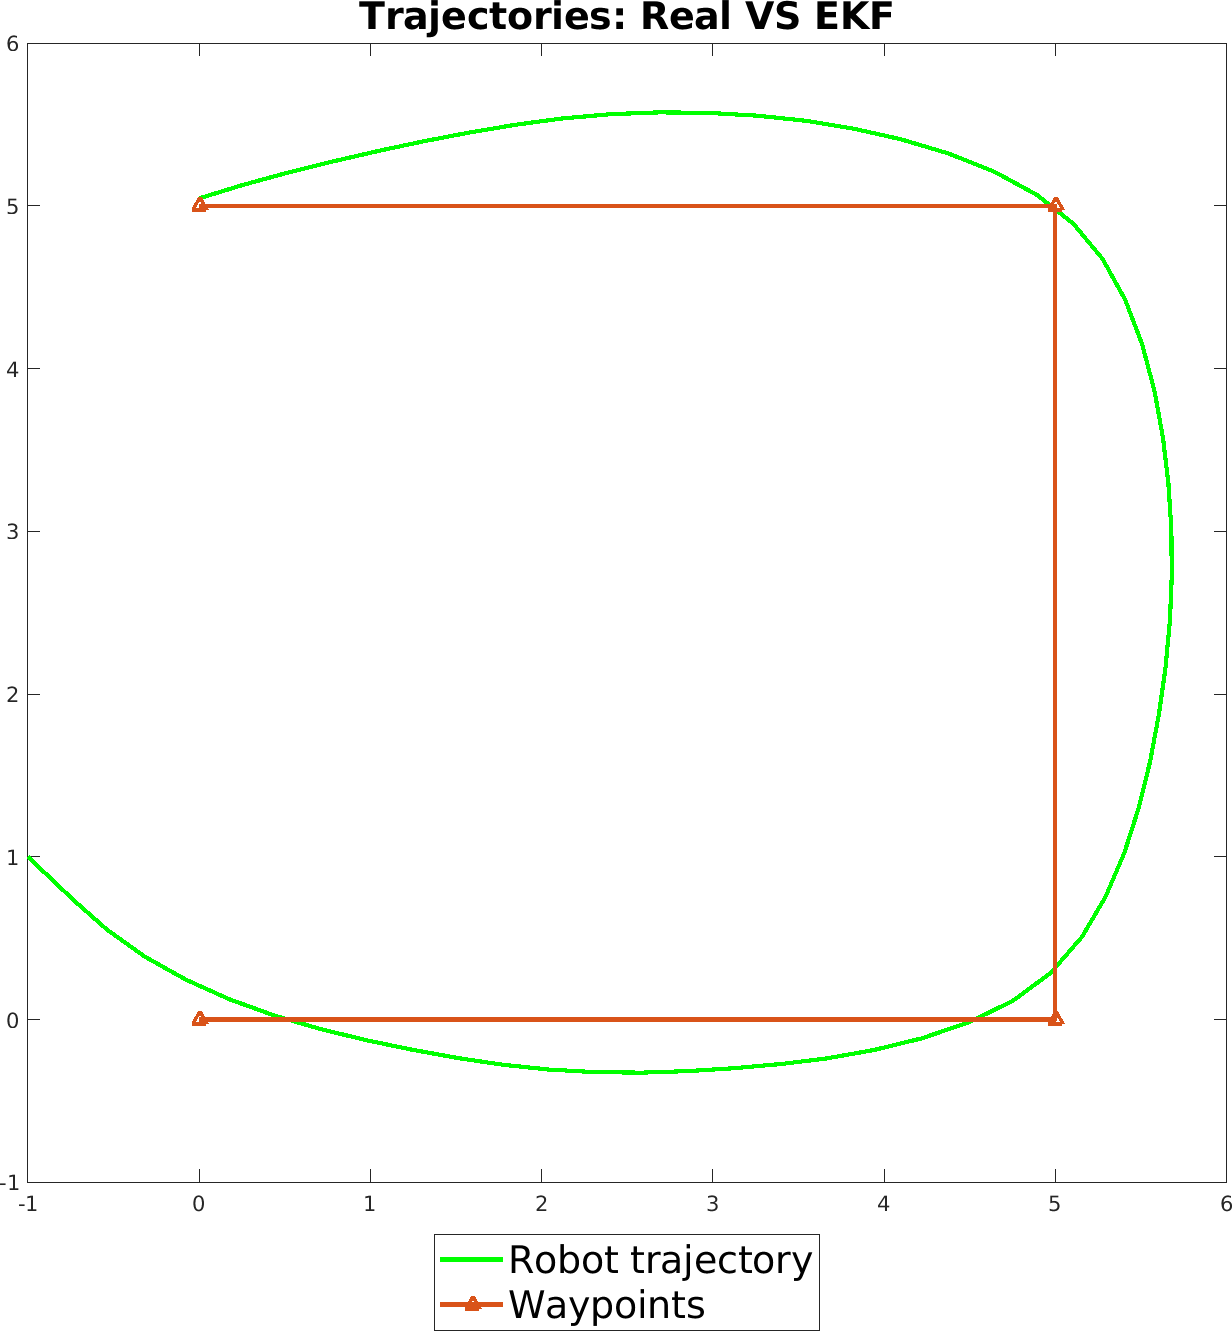
\includegraphics[width=8.5cm]{"../Report_images/Trajectory_no_EKF.png"}
    \caption{Resulting trajectory of the agent without using EKF.}
    \label{fig:EKF_off}
\end{figure}
\newpage
\begin{figure}[h!]
    \centering
    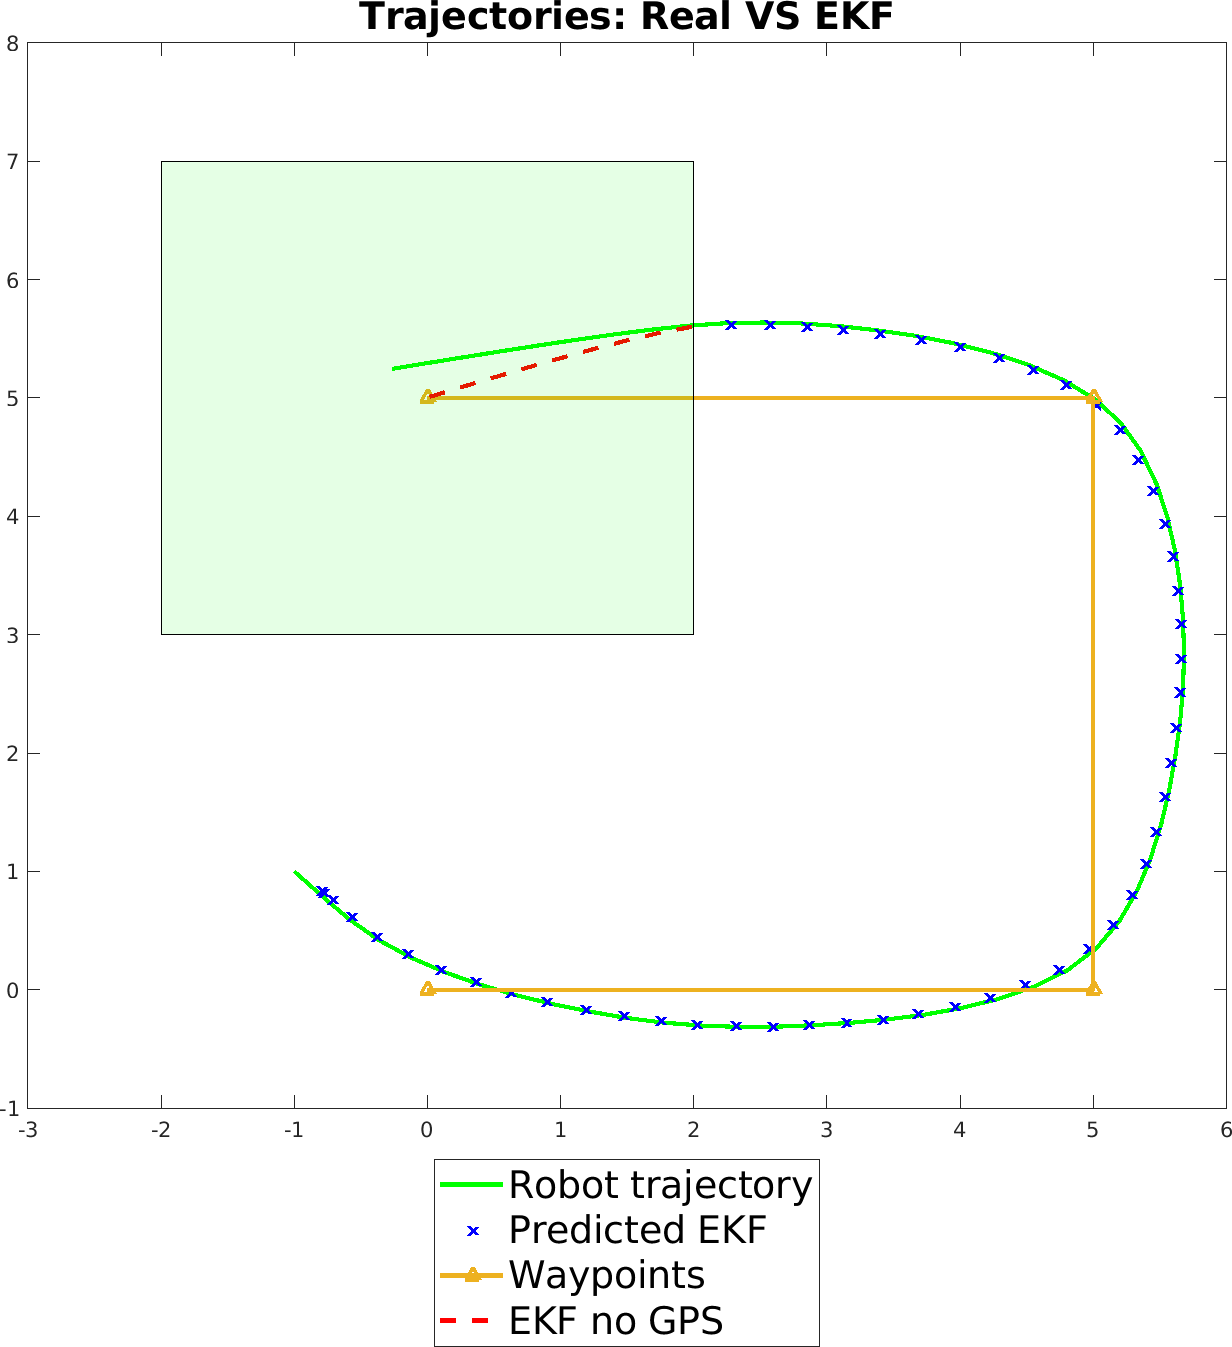
\includegraphics[width=8.5cm]{"../Report_images/Trajectory_EKF.png"}
    \caption{Resulting trajectory using EKF, red dotted, in a not GPS covered
             area, green polygon, with the estimated locations with the GPS,
             blue crosses.}
    \label{fig:EKF_on}
\end{figure}
\vspace{0.3cm}
As we can observe the agent without using the Extended Kalmann Filter carries
out its task flawless, while using it results into an overshooting of the
target due to its mismatch between the estimated location and the real one.
The first idea is that the filter has fitted only a straight line which
departs from the orientation of the robot when it enters in the area without
GPS. We firstly supposed that this behaviour was due to a poor tuning of the
filter parameters, especially of the process noise matrix which has an 
mportant role in fitting non-linearities, but after several test the
results were not getting any better. On the other hand using only the
kinematic model which composes the state transition function will lead
to good results.

\section{Conclusions}
In this report we have presented a solution to perform the Disributed SLAM
on a natural environment exploiting terrestrial agents which uses as onboard
sensors only a 3D Lidar, a gyroscope, an accelerometer and a proximity sensor.
The agents are allowed to share data whenever they are within a communication
range between each others.
% The data shared consists of the 3D point cloud,
% the 2D occupancy map and the pose updated up to that moment. After the
% sharing each agent updates its inner representation of the surroundings
% and carries on with the exploration task.
The data from the Lidar have been corrected using a Linear Kalmann Filter,
while the location of the agent have been estimated using an Extended
Kalmann Filter whenever a reliable GPS location was not available.
Our approach provided satisfactory results in the estimation of the 
data but performed poorly in estimating the absolute pose with the extended
filter.

\subsection{Benefits and Limits}
Our approach resulted proficient even if the amount of sensors onboard is
reduced, but this may result in cheaper applications where the highest
amount of the expense is due to the lidar sensor.
Unfortunately its inability in estimating correctly its position in absence
of GPS data consists in a huge flaw which can lead to unrecoverable states
during the exploration.
Furthermore, the system is subjected to blind spots in the Lidar point
cloud due to the pits in the terrain as shown in Figure \ref{fig:cloud_pits}
being the agent nerby the edge of a cliff.
This issue may be easily solved by moving the Lidar sensor in a slightly
inclined position facing the ground or even adding a second lidar with
a restricted FoV, lastly it is possible to act passively on the problem
by reducing the movement distance for the robot and forcing it to acquire
more data in despite of the memory requirements and time for the mapping.

\subsection{Future Directions}
% Considerations about using the intensity of the lidar beams -> water
In the future it should be taken into consideration the presence of water
basins, ponds or any other elements containing water in the surroundings which
may be seen as flat surfaces by the laser inside the Lidar, due to the highly
reflectance of the water. Knowing this it should be possible to detect the
threat represented by the water by analyzing the intensity of the beam
returned to the sensor.
Another expansion for this project could be the definition of more advanced
classification algorithms to detect the points representing ground, maybe
using SVM or other machine learning techinques for classification.
In the end a fix to the Extended Kalmann Filter estimation or an
alternative solution must be explored.

\vfill
\footnotesize{
    The authors have the following addresses: Italy\newline
    \small{\{\texttt{davide.bertelli-1,jhonny.hueller}\}%
             \texttt{@studenti.unitn.it}.}
    \footnotesize{
    This report is the final document for the course of “Distributed Systems
    for Measurement and Automation”.}
}

\newpage
\section{Additional Materials}
\begin{figure}[!h]
    \centering
    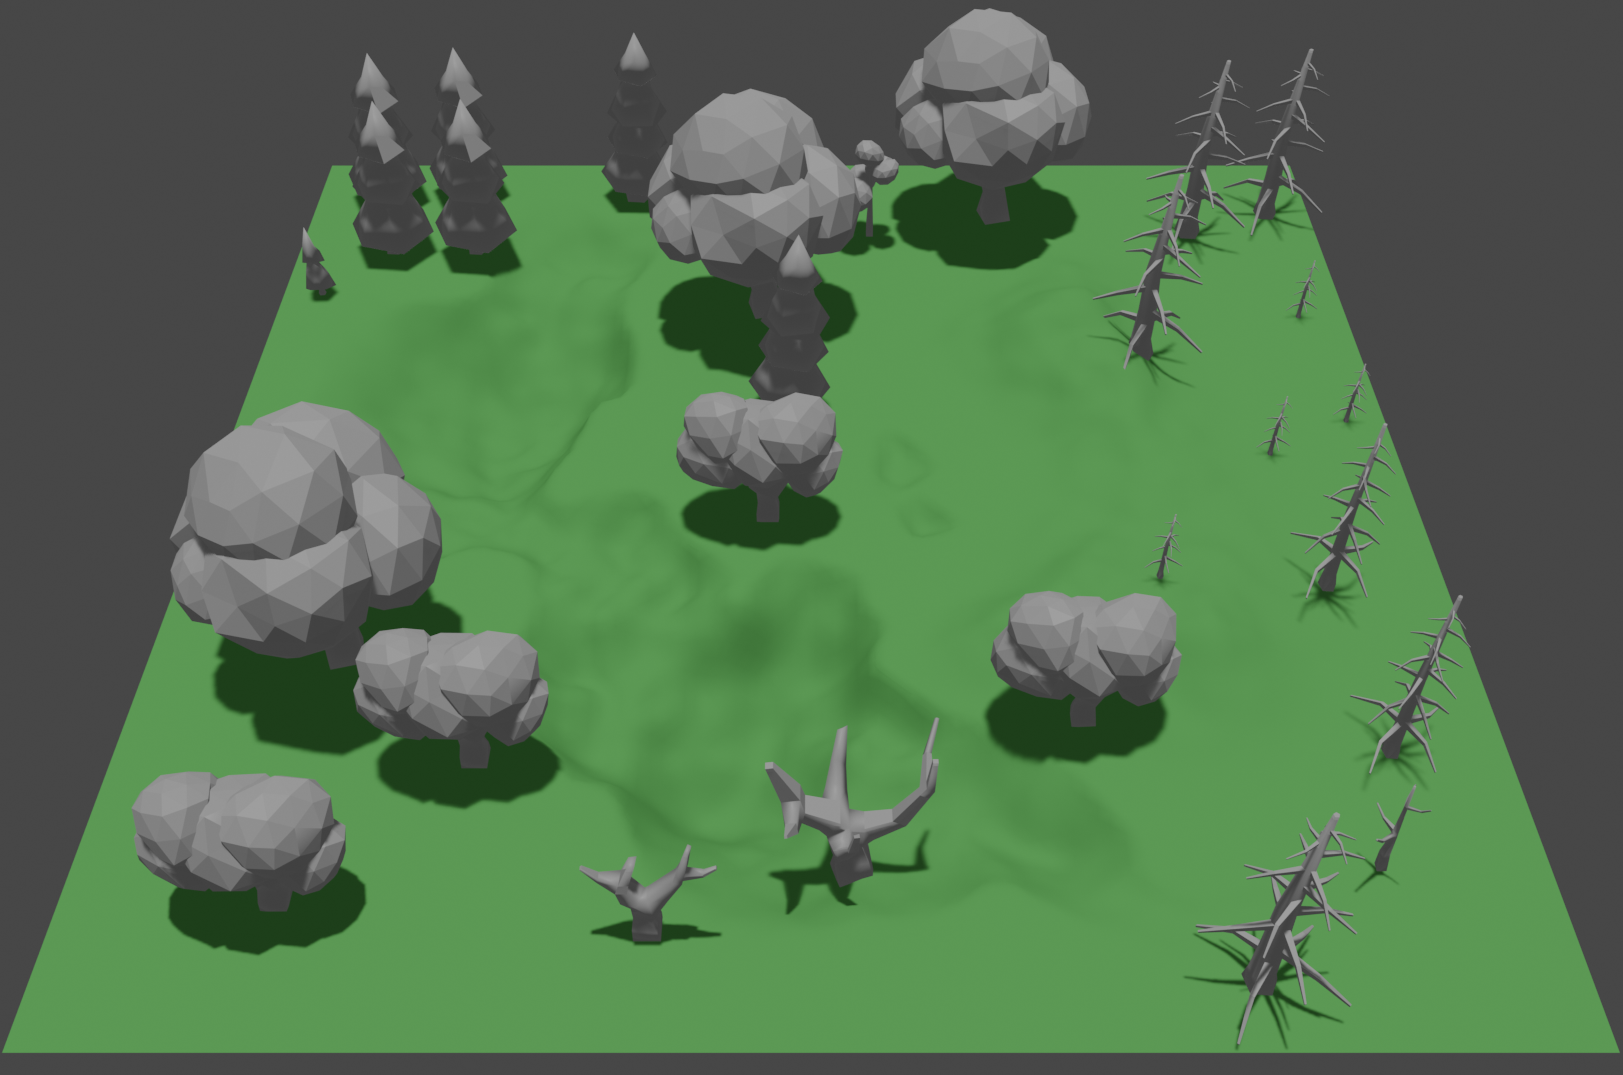
\includegraphics[width=18cm]{"../Report_images/World.png"}
    \caption{Full image of the simulated world with pits.}
\end{figure}

\end{document}
